\chapter{Population Health \& Climate Heating}
\openepigraph{%
	A ruined planet cannot sustain human lives in good health. A healthy planet and healthy people are two sides of the same coin.
}{Dr. Margaret Chan, Executive Director, WHO}

\marginnote{
	\newthought{Key Message:} The impact of climate heating on local populations is a truly wicked problem that public health practitioners spend very little time thinking about. It's too hard. It isn't a health system priority; it is tomorrow's problem. We need to make it easier to understand and incorporate into all local population planning. Systems thinking might provides some useful tools.
}

\section{Complexity and Public Engagement}
The aim of this document is to bring together all threads of this project that set out to explore how public health could develop policy in the area of potential health impacts from climate change on the older population of West Dorset. It became obvious quite early in the project that this was not going to be an easy task. The difficulty arises firstly in developing a meaningful engagement on the topic. Getting attention for a problem that is in the future, and not thought to be more significant in impact than many current population health issues was always going to be a challenge.

We have approached this challenge by adopting a `systems thinking' approach to our engagement with policy makers and `futures studies' approach in our engagement with the community more widely. In truth, these approaches are complementary and underpin both engagement processes.

\begin{description}
	\item[Systems Thinking]An approach to developing deeper understanding of complexity by examining problems and challenges within the context of the `system' in which they exist.
	\item[Futures Studies] An approach to the development of strategy that seeks to understand an issue or challenge in the context of a more comprehensive picture of a future state. Incorporates a fundamental belief that at any point in time there are many possible futures -- strategically one should work towards a preferred future.
\end{description}

\subsection{Change of Project Emphasis}
The project that began as a climate change impacts on the health of older persons in West Dorset, ended as a project entitled, \emph{Complex Challenges \& Public Engagement}, reflecting the broader issues we encountered during the running of this project.

Our change in emphasis was not an abandonment of the initial research focus that sought to develop a better understanding of what impacts older people in West Dorset would face in thirty years. Indeed, it was our desire to make a meaningful contribution in this area that we realised that our initially more traditional research approach had two shortcomings:
\begin{enumerate}
	\item Scientific uncertainties regarding the estimated outcomes 30 years in the future are such that we would not succeed in delivering new information, but rather our approach would include the same lists of possible outcomes and generalised mortality outcomes; and
	\item Consequently, the initial difficulties we experienced in engaging stakeholders would be compounded, because we had nothing particularly compelling to engage with.
\end{enumerate}

\subsection{Project Outputs}
Thus far this project has presented a number of workshops, a conference poster and delivered a systems model and story, various futuring deliverables including a Futures Story and this report.

It is anticipated that these materials will be used further in 2016 to continue exploring the public health challenge faced by climate change in Dorset and we will also seek to publish some of this work.

Furthermore, a longer term outcome will require a longer effort as we attempt to apply the methods explored here to other public health challenges over the coming years.

\subsection{Project Outcomes}

Ultimately, Public Health Dorset role is to protect and improve the health of its population -- we hope that methods adopted during this project will contribute towards the success of that role. However, a more immediate outcome has been the exposure of many staff to systems thinking and futuring methods, which now extends their potential reach in developing shared understanding of particularly complex public health challenges.

\subsection{Report Organisation}

Part I of this report focusses on the `systems thinking', `systems modelling' and `systems story telling' methods that were used in an effort to develop a shared understanding of this public health challenge.

Part II reports on the use of future methods: `horizon scanning', `scenario building' and `futures story telling'.

Part III of this report serves as a repository for presentations and stakeholders events, recording the evolution of the group's thinking over the two year life of the project.

\section{Public Health and Systems Thinking}
Systems Thinking as an approach to problem solving appears to have evolved from a sub-discipline of Engineering, Systems Dynamics, and the work of Jay Forrester.\cite{WikipediaJWF} However, it has been used more broadly to explore problems in natural systems, business and organised problem solving more generally.\cite{Ford2010, Senge2006, MaaniCavana2007}

The articulation of systems thinking as a tool in the practice of public health has only occurred relatively recently in explicit reference to `systems', ``The whole concept of public health is founded on the insight that health and illness have causes or conditions that go beyond the biology and behaviour of the individual human being''.\cite{Midgley2006} While, this has always been implicitly understood in modern public health, 

\begin{quotation}
\ldots there is no single operational method for identifying and interpreting these relationships, there is, in fact, a common conceptual orientation recognizable as a systems approach: it is a paradigm or perspective that considers connections among different components, plans for the implications of their interaction, and requires transdisciplinary thinking as well as active engagement of those who have a stake in the outcome to govern the course of change.\cite{Leischow2006}
\end{quotation}

It is clear that a systems approach is intuitively sensible and that the methods available have matured to make its adoption in public health practice both timely and practicable.\cite{Trochim2006, Homer2006} Nonetheless, we still to this day have relatively few examples of its use at the `coal face', and the authors of these works are academics and management consultants.

More recent work looking at the use of a systems approach in disentangling health disparities and health system policy are aimed at experts in their respective fields and not at developing a shared understanding of the public health challenge to public health practitioners.\cite{Roux2011} Indeed, one could question the degree to which these authors truly understand sytems thinking and the application of causal loop and other methods when talking of `health systems' and making only the most rudimentary attempt to actually visualise and map the system.\cite{BoschCapblanch2012} Nonetheless, the effort to improve the targeting of these methods and make a difference in public health continues,

\begin{quotation}
Recognizing that a problem exists and taking action to solve a problem are two activities that many do well, but there is an in-between step that often receives inadequate attention. The source of all important management blunders can be traced back to a mistake in accurately discerning what is important in a situation and incorrectly formulating a problem to be addressed.\cite{Canyon2013}
\end{quotation}

\section{Health Impacts of Climate Change on an Ageing Population}

With this background of a rather recent and not-so-successful introduction of public heath to systems thinking methods, we have focussed on a systems approach because it seemed the only way to adequately address this problem in a way that would make meaningful communication with all stakeholders possible.

\subsection{The Big Picture}
There is a scientific consensus that anthropogenic climate change is increasing global temperature and that this will continue for at least another century. This will impact human health and well-being because the links to human health and climate are well understood.

\begin{quotation}
The health of human populations is sensitive to shifts in weather patterns and other aspects of climate change (very high
confidence). These effects occur directly, due to changes in temperature and precipitation and occurrence of heat waves, floods, droughts, and fires\ldots Until mid-century climate change will act mainly by exacerbating health problems that already exist (very high confidence)\ldots (p. 713)\cite{IPCC2014}
\end{quotation}

The impact of climate change on older persons will be particularly problematic, because

\begin{quotation}
Older people are also more likely to suffer from health conditions that limit the body's ability to respond to stressors such as heat and air pollution\ldots (p. 718)\sidenote{Citation as above.}
\end{quotation}

The range of potential health impacts identified is lengthy and includes:\cite{Portier2010}
\begin{itemize}
\item Asthma, Respiratory Allergies, and Airway Diseases
\item Cancer
\item Cardiovascular Disease and Stroke
\item Foodborne Diseases and Nutrition
\item Heat-Related Morbidity and Mortality
\item Human Developmental Effects
\item Mental Health and Stress-Related Disorders
\item Neurological Diseases and Disorders
\item Vectorborne and Zoonotic Diseases
\item Waterborne Diseases
\item Weather-Related Morbidity and Mortality
\end{itemize}

There have been numerous substantial reviews on the potential health impacts of climate change on the human population and potential mitigation strategies from the WHO\cite{WHO2014a,WHO2014b, WHO2015}, the IPCC\cite{IPCC2014}, the US\cite{Portier2010, Luber2014} and the UK\cite{HPA2012, LancetCom2015}.


The general consensus is that climate change will impact human health in a myriad of ways in the not distant future and that the focus should now turn to mitigation of health impact. There does not, however, appear to be a simple recipe that can be applied and the consequences for much of the developing world will be far more severe than that in the developed world. Nonetheless, scientific evidence suggests that the impacts will be severe and measurable.


\subsection{Temperature Stress Attributable Excess Mortality}
Temperature stress to human physiology, both cold and warm, is relative to whatever is considered to be a 'normal' temperature range. It is important to emphasise that excess mortality related to cold and warm temperature stress is evident at very average temperatures. A recent English study indicates that local temperature stresses occur over very average temperature ranges.\cite{Hajat2014}

In Dorset, UK, temperature stress is estimated to occur when it is either warmer than 17.6 deg C or cooler than 12.1 deg C. The relative risk (RR) of death increases by approximately 2\% for each degree C beyond these thresholds (Figure~\ref{fig:rr}).

As a consequence of Dorset's ageing population, excess winter mortality in the Southwest will continue to be far more of a problem than excess heat related deaths even in a warmer world of 2044. This counter-intuitive finding is entirely driven by the demographic trend of an ageing population.


\begin{figure}[htbp]
\centering
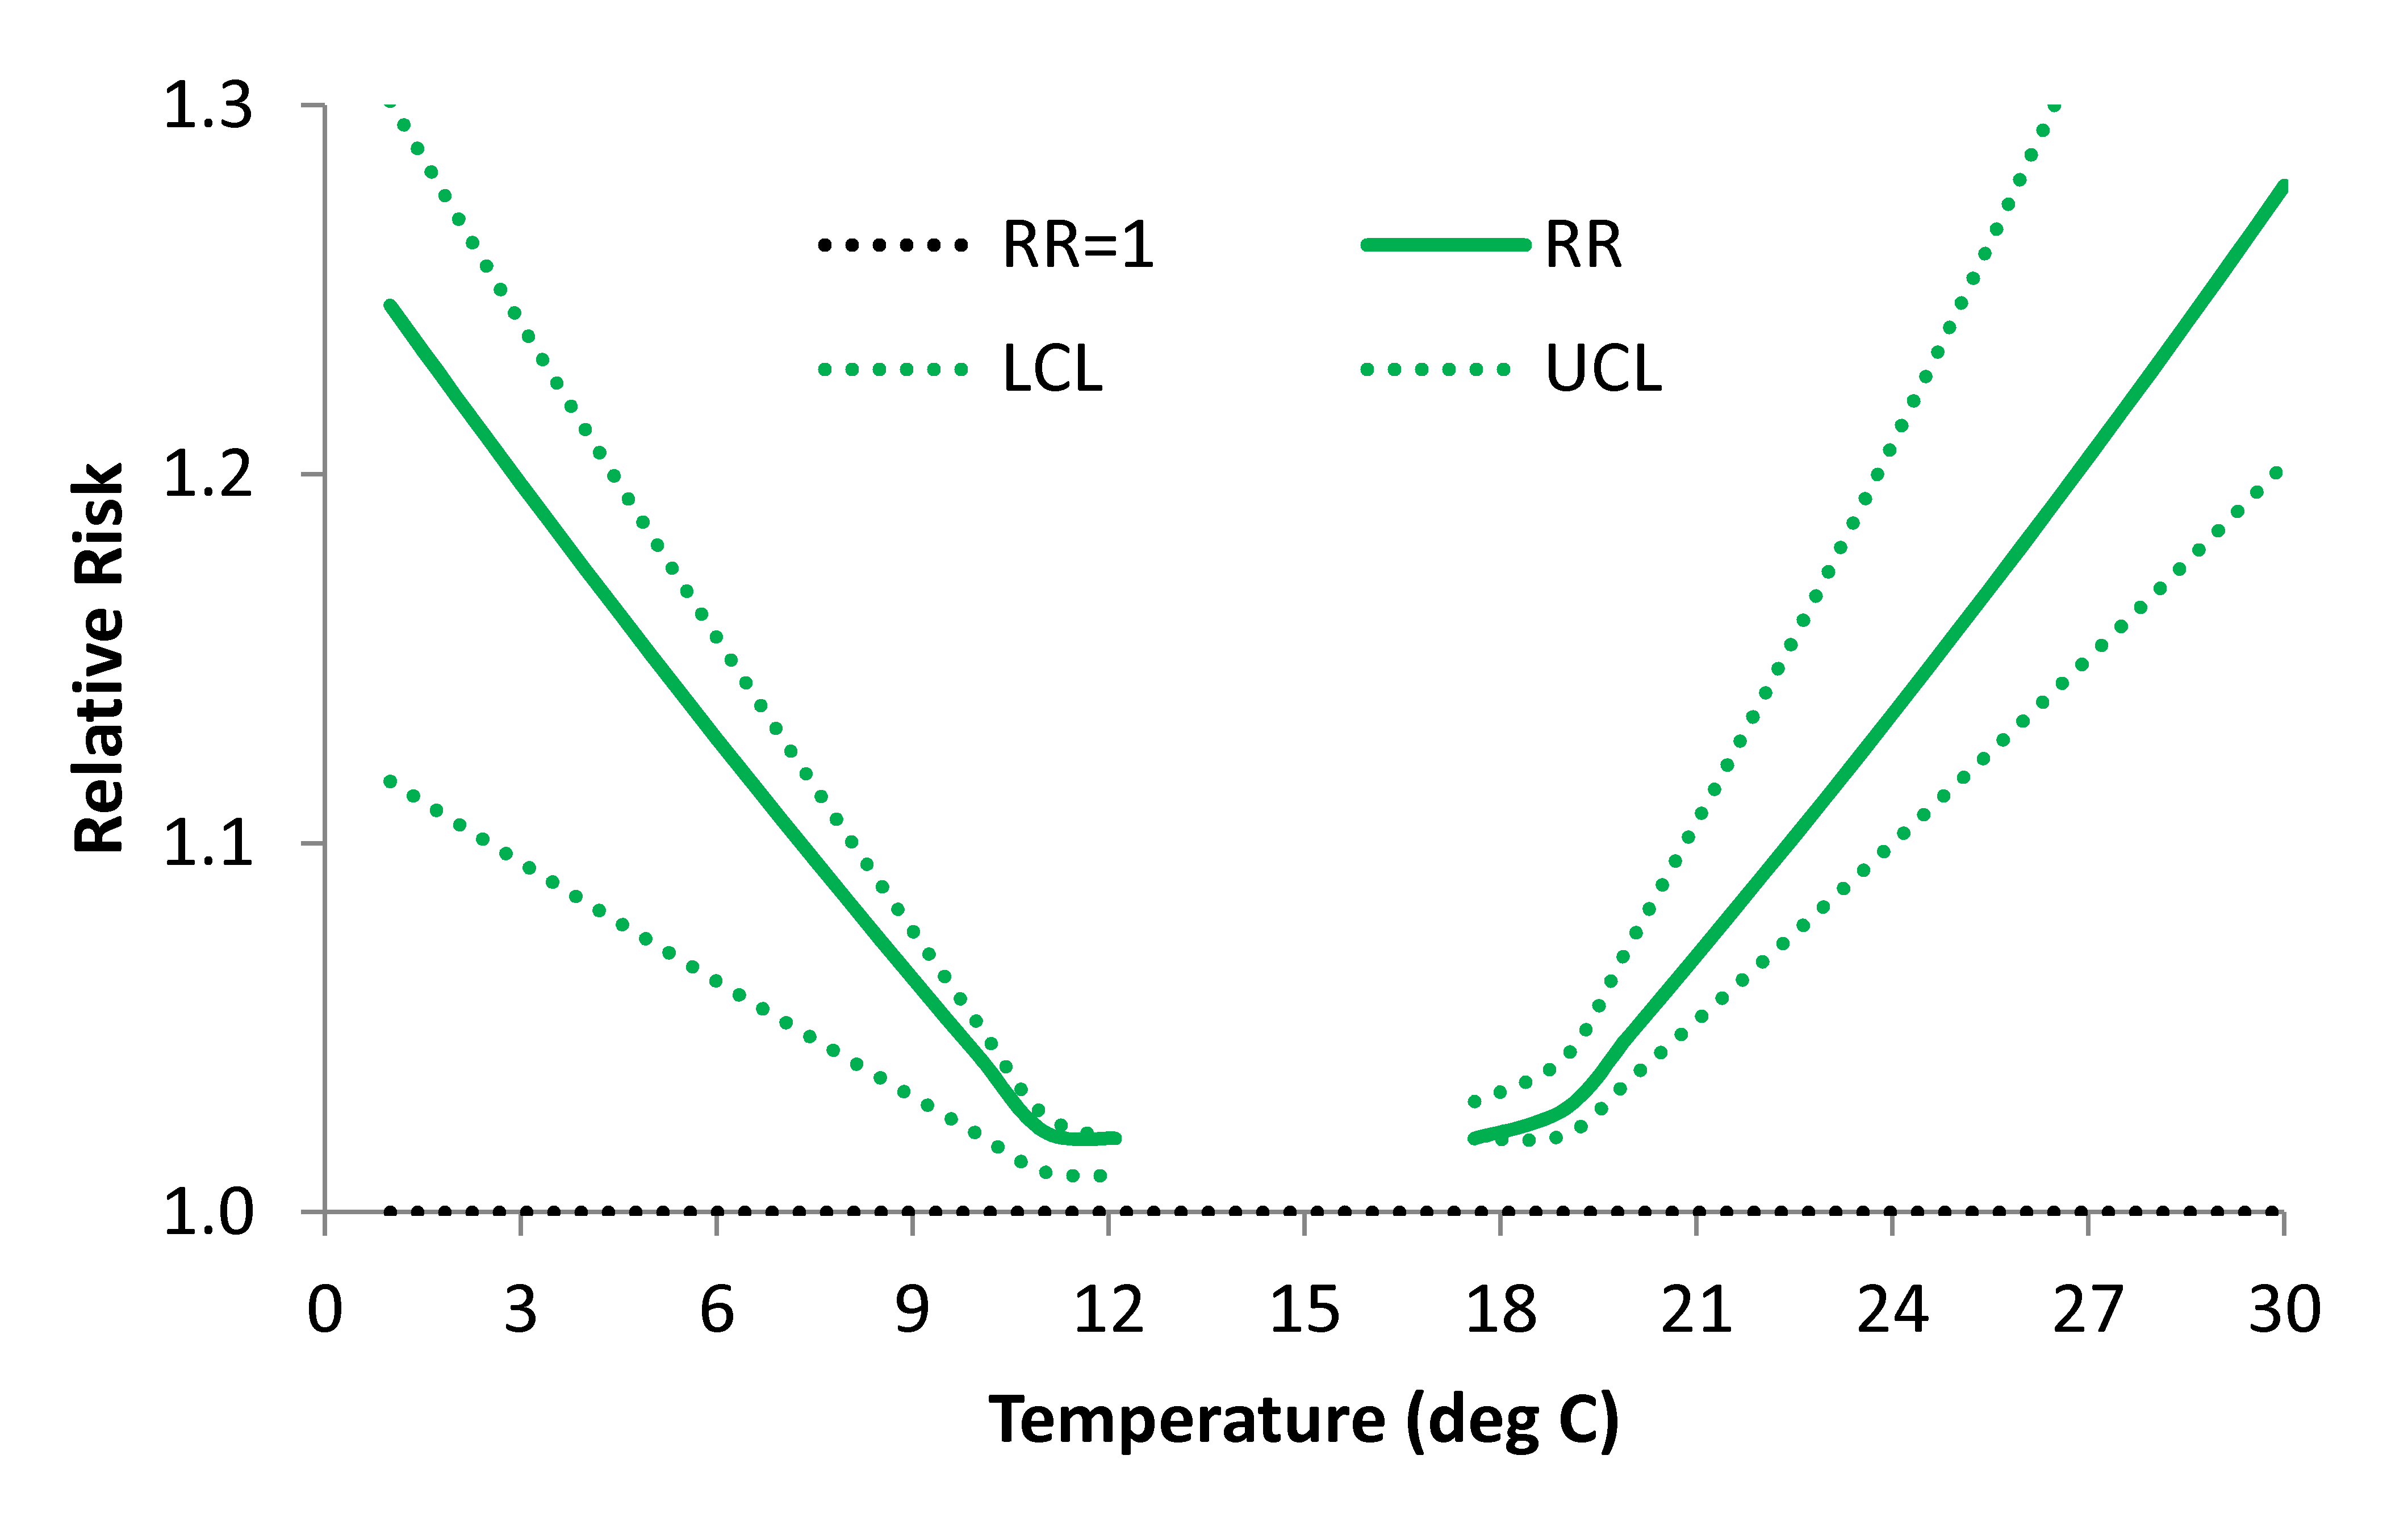
\includegraphics{CCA/img/RRgraph.png}
\caption[Relative Risk and Temperature]{The relative risk (RR) of death increases by approximately 2\% for each degree C beyond these thresholds.\label{fig:rr}}
\end{figure}





\section{Climate Change}
\subsection{Climate Change Projections for UK}
This simulation model is based upon \href{http://ukclimateprojections.metoffice.gov.uk/media.jsp?mediaid=87867 \&filetype=pdf}{UKCP09 SRES A1B Emission Scenario Projection}, which "provides a basis for studies of impacts and vulnerability and decisions on adaptation to climate change in the UK over the 21st century."\cite{Jenkinsetal2009}

The emission 'story line' that underpins the future climate scenario used in this work is the IPCC's  \href{http://www.grida.no/publications/other/ipcc_sr/?src=/climate/ipcc/emission/}{Special Report Emissions Scenarios}.\cite{IPCC2000}

The Weather Generator is used here to provide a time series of mean daily temperature. It allows users to generate plausible daily time series at 5 km resolution level. As there is no climate change data available at the 5km scale, the Weather Generator 'downscales' the climate data from the 25km scale (Figure~\ref{fig:wgd}).\cite{Jonesetal2010}

\begin{figure}[htbp]
\centering
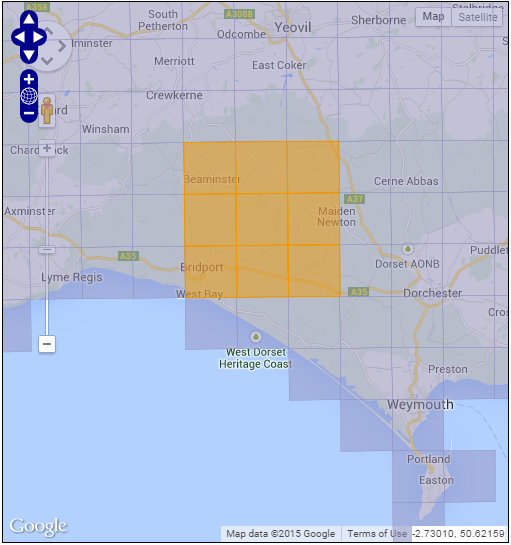
\includegraphics{CCA/img/WGD_WD.png}
\caption{Weather Generator spatial resolution over the West Dorset region.\label{fig:wgd}}
\end{figure}




\section{Ageing Population}



\subsection{West Dorset Situation}
Dorset's population is ageing and this will have be a factor in how severely population health will be impacts by changing climate over the next 30 years. Population ageing, meaning that there will be a greater proportion of the population that is older in the future than is currently the case, is a global trend across the developed western world including the UK. There is a high degree of certainty that this trend will continue well beyond the 30 year reach of this study.

2012-based \href{www.ons.gov.uk/ons/rel/snpp/sub-national-population-projections/2012-based-projections/index.html}{Sub-national Population Projections} for Local Authorities in England, by sex and 5 year age groups, all local authorities and higher administrative areas within England Long-term sub-national population projections are an indication of the future trends in population by age and sex over the next 25 years.\cite{ons2012} They are trend-based projections, which means assumptions for future levels of births, deaths and migration are based on observed levels mainly over the previous five years. They show what the population will be if recent trends continue.

There are a number of uncertainties in ageing and the future of ageing in 2044 that we need to think carefully about:
\begin{itemize}
\item Quality of life, including increased fitness levels
\item Future work/retirement balance
\item Isolation and support for older people
\end{itemize}

\section{Public Health Interventions}
All public health interventions can be defined by three characteristics: the reach of the intervention (ie. who gets access to the intervention), who complies with the intervention, and what is the efficacy of the intervention.





